\documentclass[11pt,a4paper]{article}

\usepackage[utf8]{inputenc}
\usepackage[T1]{fontenc}
\usepackage[spanish,es-nodecimaldot]{babel}
\usepackage{lmodern}

\usepackage{graphicx}
\usepackage{geometry}
\usepackage{array}
\usepackage{amsmath}
\usepackage{titlesec}
\usepackage{hyperref}
\usepackage{fancyhdr}

\usepackage{booktabs}
\usepackage{float}

\fancyhf{}

\fancyhead[L]{\small\textit{Universidad Nacional de Ingeniería}}
\fancyhead[R]{\small\textit{2026--II}}
\renewcommand{\headrulewidth}{0.4pt}
\fancyfoot[C]{\thepage}

\geometry{
    top=2.2cm,
    bottom=1.5cm,
    left=2.5cm,
    right=2.5cm,
    headheight=14pt,
    headsep=0.5cm
}

\setlength{\parindent}{0pt}
\setlength{\parskip}{0.5em}
\pagestyle{plain}
\setcounter{secnumdepth}{2}
\setcounter{tocdepth}{2}
\addto\captionsspanish{%
    \renewcommand{\contentsname}{Contenido}%
}
\hypersetup{
    colorlinks=true,
    linkcolor=black,
    citecolor=black,
    urlcolor=blue
}

\titlespacing*{\subsection}
    {0.6cm}
    {1.5em}
    {0.8em} 

\newenvironment{subsectionbody}
{%
    \begin{list}{}{%
        \setlength{\leftmargin}{0.6cm}%
        \setlength{\rightmargin}{0cm}%
        \setlength{\topsep}{0pt}%
        \setlength{\partopsep}{0pt}%
        \setlength{\parsep}{0pt}%
        \setlength{\itemsep}{0pt}%
    }%
    \item\relax
}
{%
    \end{list}
}

\setcounter{secnumdepth}{3}

\titlespacing*{\section}
{0pt}{12pt}{8pt}

\titlespacing*{\subsection}
{0.5cm}{10pt}{6pt}

\titlespacing*{\subsubsection}
{1cm}{8pt}{5pt}

\begin{document}

\begin{titlepage}

\thispagestyle{empty}

\begin{center}
{\normalsize\itshape
``Año de la Recuperación y Consolidación de la Economía Peruana''}

\vspace{0.35cm}
\resizebox{0.68\textwidth}{!}{%
    \textbf{Universidad Nacional de Ingeniería}%
}

\vspace{0.30cm}
{\Large\bfseries
Facultad de Ciencias}

\vspace{0.35cm}
{\Large\bfseries
Física II}

\vspace{0.30cm}

\includegraphics[width=4.5cm]{../figuras/imagen_uni_escudo.png}

\vspace{0.25cm}
{\Large\bfseries
Laboratorio 4}

\vspace{0.35cm}
{\Large\bfseries\itshape
Tensión superficial}
\end{center}

\vspace{1.15cm}
\noindent
\begin{tabular*}{\textwidth}
{@{\extracolsep{\fill}}ll}
{\large\textbf{Sección:} B}
&
{\large\textbf{Día y hora:} 27/10/2026 -- 1:00 p.\,m.}
\end{tabular*}

\vspace{0.90cm}
\renewcommand{\arraystretch}{1.45}
\begin{center}
{\large
\begin{tabular}{|p{9.7cm}|p{3.4cm}|}
\hline
\textbf{Apellidos y nombres}
&
\textbf{Código}
\\
\hline
Moreno Cabanillas, Alexandra Romina
&
20251764F
\\
\hline
Mauricio Andre Polak Mory
&
20250575E
\\
\hline
Pablo Mauro Cárdenas Loyola
&
20262378E
\\
\hline
\end{tabular}
}
\end{center}

\vspace{0.85cm}
{\large\textbf{Docentes:}}
\vspace{0.35cm}
{\large
\hspace{0.6cm}

-- Cortez Reyes, Gregorio Custodio
\vspace{0.20cm}
\hspace{0.6cm}

-- Silva Vásquez, Humberto Martín
}

\vspace{0.95cm}
{\large
\textbf{Fecha de entrega del informe:}
\hspace{0.40cm}
17/09/2026
}

\vspace{1.15cm}
\begin{center}
{\huge\bfseries
2026--II}

\end{center}

\end{titlepage}

\tableofcontents

\newpage
\pagestyle{fancy}

\section{Introducción}

El estudio de la tensión superficial tiene sus antecedentes
en las primeras observaciones de fenómenos capilares. Durante 
el siglo XV, Leonardo da Vinci registró el ascenso de líquidos 
en tubos estrechos, un fenómeno que posteriormente sería 
conocido como capilaridad. En 1721, Isaac Newton intentó explicar 
este comportamiento mediante las fuerzas de cohesión entre las 
moléculas del líquido y de adhesión entre el líquido y las paredes 
del tubo. 
Un avance fundamental ocurrió en 1751, cuando Johann Andreas 
von Segner propuso que la superficie de un líquido se comportaba 
como una película sometida a una tensión uniforme. Esta idea 
permitió introducir formalmente el concepto de tensión superficial. 
Posteriormente, a comienzos del siglo XIX, Thomas Young y Pierre-Simon 
Laplace desarrollaron las bases teóricas para explicar fenómenos como 
la curvatura de las superficies líquidas, la capilaridad y el equilibrio 
entre líquidos y sólidos. 


Durante el siglo XIX, los trabajos de Carl Friedrich Gauss y Josiah Willard 
Gibbs contribuyeron a interpretar la tensión superficial desde una 
perspectiva energética y termodinámica. Así, dejó de entenderse únicamente 
como una fuerza superficial y comenzó a relacionarse con la energía necesaria 
para incrementar el área de una interfaz. Más adelante, los estudios de Lord 
Rayleigh y otros investigadores ampliaron la comprensión de las interacciones 
moleculares responsables de este fenómeno. 

Con el desarrollo de nuevos instrumentos y procedimientos experimentales, 
fue posible medir la tensión superficial con mayor precisión. Entre los 
métodos que se consolidaron se encuentran el de la placa de Wilhelmy y 
el del anillo de du Noüy, que permiten determinarla a partir de las 
fuerzas ejercidas sobre elementos en contacto con la superficie de un 
líquido. Estos avances sentaron las bases de las técnicas experimentales 
utilizadas actualmente en física, química e ingeniería.

En la presente experiencia se busca determinar
experimentalmente el coeficiente de tensión superficial
del agua mediante la implementación de un equipo de Leybold
nos permitira registra la fuerza en función del tiempo, 
y a partir de esa fuerza podemos calcular el coeficiente 
de tensión superficial.

De esta manera, se busca analizar el comportamiento
de las superficies líquidas y comparar los resultados
obtenidos mediante ambos métodos experimentales.

\newpage
\section{Objetivos}

\subsection*{Objetivo General}
Determinar experimentalmente el coeficiente de tensión superficial del agua y de una solución de agua con detergente, mediante la implementación del método del anillo de Du Noüy utilizando un sensor de fuerza digital (Leybold).

\subsection*{Objetivos Específicos}
\begin{itemize}
    \item Analizar el comportamiento de la fuerza registrada por el sensor en función del tiempo, identificando las etapas de inmersión, formación de la película líquida, fuerza máxima (punto de ruptura) y fuerza final.
    \item Calcular el coeficiente de tensión superficial (\(\gamma\)) para ambas muestras (agua pura y agua con detergente), aplicando la ecuación teórica del método del anillo y utilizando las dimensiones geométricas del anillo medidas con el calibrador.
    \item Comparar los resultados experimentales obtenidos entre el agua pura y la solución con detergente, para evidenciar cuantitativamente el efecto de los agentes tensioactivos (reducción de la tensión superficial).
    \item Evaluar las posibles fuentes de error o discrepancias entre los valores experimentales obtenidos y los valores teóricos reportados en la literatura, considerando factores como la limpieza del anillo, las fuerzas dinámicas por la velocidad de elevación y la presencia de vibraciones externas.
\end{itemize}


\newpage
\section{Fundamentos teóricos}

\subsection{Tensión superficial y fuerzas intermoleculares}

``Las fuerzas que mantienen unidas a las moléculas de un líquido se denominan fuerzas de cohesión. En el interior del líquido, una molécula está rodeada por otras en todas direcciones, por lo que la fuerza neta sobre ella es cero. Sin embargo, en la superficie, las moléculas solo experimentan atracción hacia el interior del líquido, lo que genera una superficie que se comporta como una membrana elástica estirada.''

\begin{flushright}
Young y Freedman, \textit{Física universitaria}, pág. 424
\end{flushright}

\subsection{Deducción de la ecuación para hallar la tensión superficial}

Para determinar el coeficiente de tensión superficial (\(\gamma\)) por el  método del anillo de Du Noüy, es necesario analizar las fuerzas que actúan sobre el anillo en el momento exacto en que la película líquida está a punto de romperse.

Cuando el anillo se eleva, la fuerza que ejerce el sensor (\(F_{max}\)) debe equilibrar dos fuerzas: el peso del anillo en el aire (\(P_{anillo}\)) y la fuerza vertical ejercida por la tensión superficial del líquido (\(F_\gamma\)). Por lo tanto, en el equilibrio:
\begin{equation*}
    F_{max} = P_{anillo} + F_\gamma
\end{equation*}

La fuerza de tensión superficial se distribuye a lo largo de todo el perímetro de contacto. Dado que el líquido moja tanto la cara interior como la cara exterior del anillo, la longitud efectiva de contacto es el doble del perímetro del anillo (\(2L\)). La fuerza de tensión superficial se define como:
\begin{equation*}
    F_\gamma = \gamma \cdot 2L
\end{equation*}

Donde el perímetro total \(L\) está dado por la suma de las circunferencias interna y externa:
\begin{equation*}
    L = \pi \cdot d_{ext} + \pi \cdot d_{int} = \pi(d_{ext} + d_{int})
\end{equation*}

Sustituyendo la ecuación (3) en la ecuación (2), y luego despejando la fuerza de tensión, obtenemos:
\begin{equation*}
    F_\gamma = \gamma \cdot 2\pi(d_{ext} + d_{int})
\end{equation*}

Finalmente, reemplazando esta expresión en la ecuación de equilibrio (1) y despejando el coeficiente de tensión superficial \(\gamma\), obtenemos la ecuación que se utilizará en la sección de cálculos:
\begin{equation} \label{eq:tension_superficial}
    \gamma = \frac{F_{max} - P_{anillo}}{2\pi(d_{ext} + d_{int})}
\end{equation}
donde:
\begin{itemize}
    \item \(\gamma\): coeficiente de tensión superficial, en N/m.
    \item \(F_{max}\): fuerza máxima registrada por el sensor antes de la ruptura, en N.
    \item \(P_{anillo}\): peso del anillo seco en el aire, en N.
    \item \(d_{ext}\): diámetro exterior del anillo, en m.
    \item \(d_{int}\): diámetro interior del anillo, en m.
\end{itemize}

\subsection{Propagación de incertidumbres}

En toda medición experimental, los valores obtenidos están sujetos a incertidumbres instrumentales y aleatorias. Cuando una magnitud física (como la tensión superficial \(\gamma\)) no se mide de forma directa, sino que se calcula a partir de otras variables medidas (como la fuerza \(\Delta F\) y el perímetro \(L\)), su incertidumbre absoluta se determina mediante el método de propagación de errores \cite{guia}.

Para una función general \(f(x_1, x_2, \dots, x_n)\) que depende de varias variables independientes, la incertidumbre absoluta \(\Delta f\) se calcula mediante la suma cuadrática de las derivadas parciales:
\begin{equation*}
    \Delta f = \sqrt{\left(\frac{\partial f}{\partial x_1}\Delta x_1\right)^2 + \left(\frac{\partial f}{\partial x_2}\Delta x_2\right)^2 + \dots + \left(\frac{\partial f}{\partial x_n}\Delta x_n\right)^2}
\end{equation*}

En nuestro caso, la tensión superficial está dada por la ecuación \(\gamma = \frac{\Delta F}{2L}\). Al aplicar la propagación de errores a esta función de productos y cocientes, es más sencillo utilizar la fórmula de incertidumbre relativa:
\begin{equation*}
    \frac{\Delta \gamma}{\gamma} = \sqrt{\left(\frac{\Delta (\Delta F)}{\Delta F}\right)^2 + \left(\frac{\Delta L}{L}\right)^2}
\end{equation*}

Despejando la incertidumbre absoluta de la tensión superficial (\(\Delta \gamma\)), obtenemos la expresión final que se utilizará en la sección de cálculos:
\begin{equation} \label{eq:propagacion}
    \Delta \gamma = \gamma \cdot \sqrt{\left(\frac{\Delta (\Delta F)}{\Delta F}\right)^2 + \left(\frac{\Delta L}{L}\right)^2}
\end{equation}
donde:
\begin{itemize}
    \item \(\Delta (\Delta F)\): incertidumbre de la fuerza neta medida (incertidumbre instrumental del sensor de fuerza).
    \item \(\Delta L\): incertidumbre del perímetro de contacto (propagada a partir de la precisión del calibrador).
\end{itemize}






\newpage
\section{Materiales y equipos}

A continuación, se detallan los elementos utilizados durante la práctica de laboratorio para la determinación de la tensión superficial.

\begin{figure}[H]
    \centering
    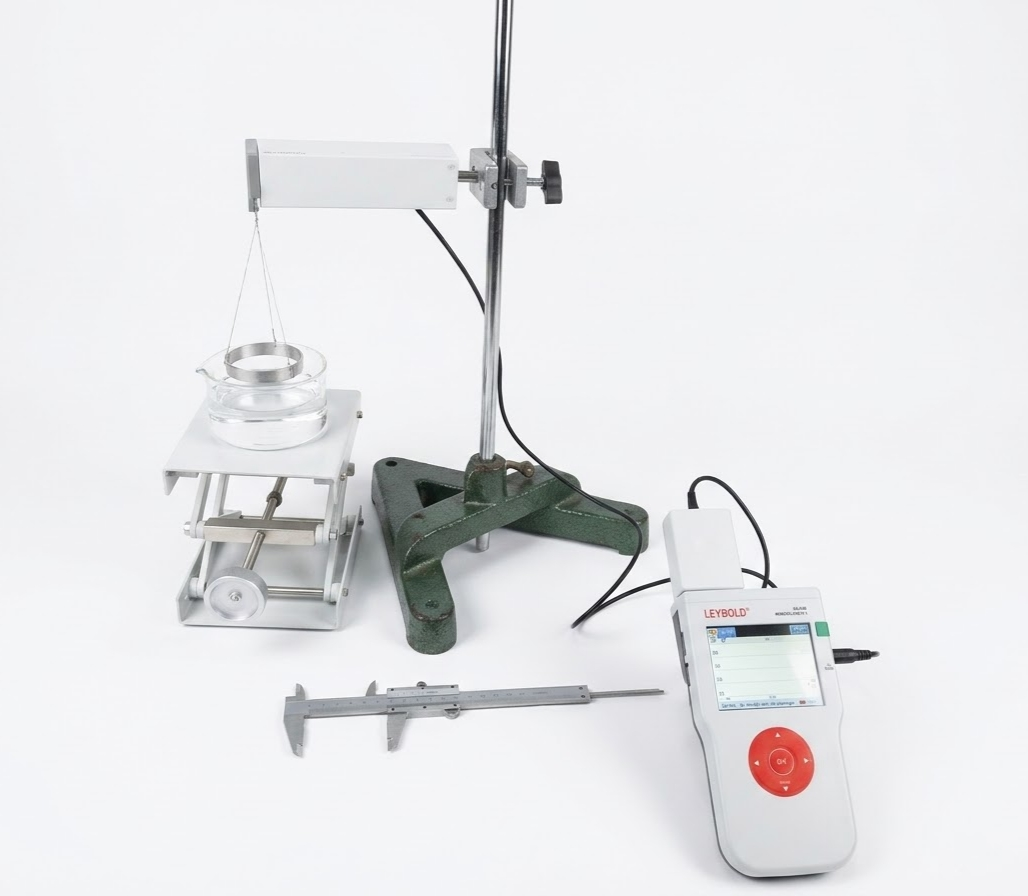
\includegraphics[width=0.85\textwidth]{../figuras/montaje.jpeg} 
    \caption{Montaje experimental para la medición de la tensión superficial .}
    \label{fig:montaje_experimental}
\end{figure}

\subsection{Elementos de montaje y soporte}

Elementos empleados para sostener el sistema de medición y permitir la elevación controlada del anillo durante la experiencia.

\begin{itemize}
    \item Soporte universal de base triangular (hierro fundido).
    \item Varilla metálica vertical y nuez de sujeción.
    \item Elevador micrométrico con mecanismo de tornillo (plataforma de elevación).
    \item Vaso de precipitados (para contener el líquido).
\end{itemize}

\subsection{Instrumentos de medición y adquisición de datos}

Instrumentos utilizados para determinar las magnitudes experimentales (fuerza, tiempo y dimensiones) y sus correspondientes incertidumbres.

\begin{itemize}
    \item Sensor de fuerza digital Leybold (Dinamómetro): Rango de medición de alta precisión, con una incertidumbre instrumental de \(\pm 0.1 \text{ mN}\).
    \item Interfaz de adquisición de datos (Cassy Lab) y computadora con software de registro.
    \item Calibrador Vernier (pie de rey): Incertidumbre instrumental de \(\pm 0.05 \text{ mm}\).
\end{itemize}

\subsection{Componentes del sistema}

Elementos que constituyen el sistema físico sometido a análisis (la interfaz líquido-aire).

\begin{itemize}
    \item Anillo metálico de Du Noüy (aleación de platino o acero inoxidable).
    \item Recipiente con agua pura (muestra 1).
    \item Recipiente con solución de agua y detergente (muestra 2).
\end{itemize}




\newpage
\section{Procedimiento experimental}

\begin{enumerate}
    \item Armé el equipo asegurando el sensor de fuerza Leybold al soporte universal y lo conecté a la interfaz Cassy Lab. Medí los diámetros interior y exterior del anillo con el vernier y registré su peso en seco.

    \item Limpié el anillo, lo suspendí del sensor y coloqué el vaso con agua pura sobre el elevador micrométrico, asegurando que el anillo quedara centrado y paralelo a la superficie.

    \item Inicié la grabación en el software y elevé lentamente la plataforma. Registré la fuerza en función del tiempo hasta que la película líquida se estiró y se rompió. Repetí la toma varias veces para observar el comportamiento del sistema y descartar curvas con exceso de ruido.

    \item Cambié el líquido por la solución de agua con detergente y repetí el proceso de inmersión y elevación. Observé que la película se estiraba mucho más antes de romperse, formando una burbuja notoria.

    \item Finalmente, de todos los registros obtenidos, seleccioné las tres curvas más contundentes (una negra, una roja y una azul) para cada muestra. Escogí las que presentaban menos perturbaciones externas y mostraban claramente el pico máximo y la ruptura, y organicé estos datos para los cálculos posteriores.
\end{enumerate}

\begin{figure}[H]
    \centering
    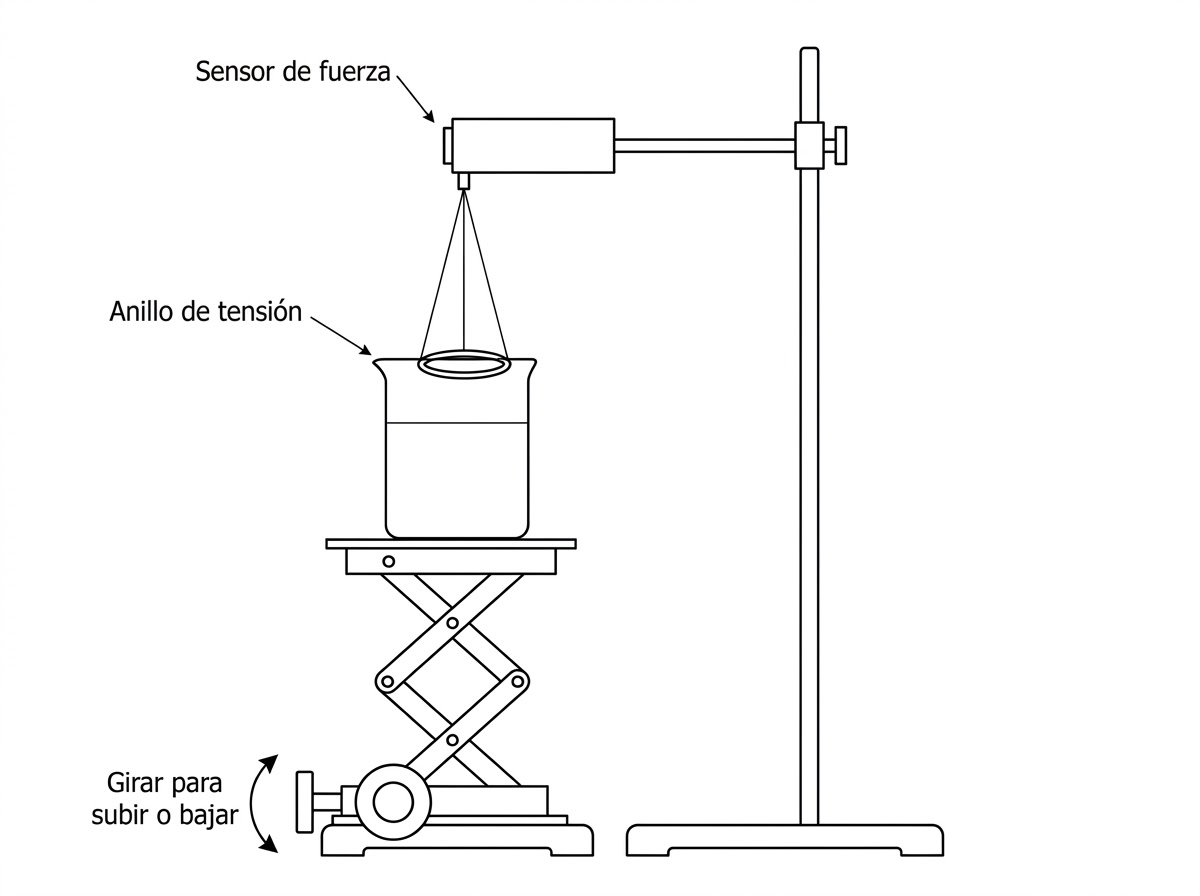
\includegraphics[width=0.7\textwidth]{../figuras/procedimiento.jpeg} % Cambia .jpeg por .png o .jpg si es necesario
    \caption{Esquema del uso del mecanismo de elevación micrométrica (tijera) para la inmersión y elevación del anillo.}
    \label{fig:esquema_procedimiento}
\end{figure}






\newpage
\section{Cálculos y resultados}
En la siguiente sección hallaremos la tension superficial
mediante el método del anillo de Du Noüy con los datos
tomados por el equipo de Leybold. Los datos registrados 
por el equipo de medicion estan adjuntadas en la carpeta
datos en el repositorio de github anexado.

\subsection{Agua con detergente}
Para esta medición, se agrego en el recipiente con agua 
una cantidad menor a 20ml de una solución, no se pudo 
precisar con detalle la cantidad exacta por ello se da un 
estimado, de agua con abundante detergente

\begin{figure}[H]
    \centering
    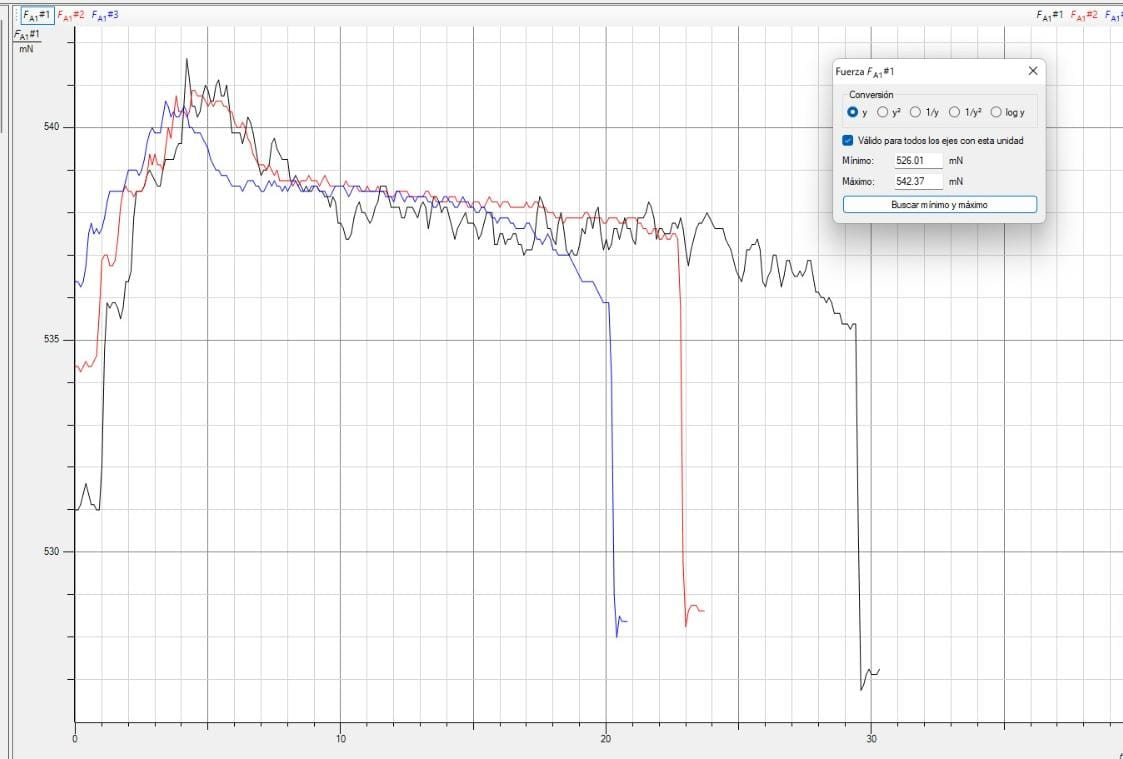
\includegraphics[width=0.8\textwidth]{../figuras/aguacondetergente.jpeg}
    \caption{Registro de la fuerza en función del tiempo para el agua pura.}
    \label{fig:grafica_agua_pura}
\end{figure}

\begin{table}[H]
    \centering
    \label{tab:parametros_anillo}
    \begin{tabular}{@{}lcc@{}}
        \toprule
        \textbf{Parámetro} & \textbf{Símbolo} & \textbf{Valor} \\ \midrule
        Diámetro exterior & \(d_{ext}\) & \(0.0596 \text{ m}\) \\
        Diámetro interior & \(d_{int}\) & \(0.0594 \text{ m}\) \\
        Perímetro de contacto & \(L\) & \(0.37385 \text{ m}\) \\
        Longitud efectiva (2L) & \(2L\) & \(0.7477 \text{ m}\) \\ \bottomrule
    \end{tabular}
    \caption{Parámetros geométricos del anillo de Du Noüy.}
\end{table}

El perímetro total de contacto \(L\) se calcula considerando que el líquido ejerce fuerza tanto en la cara interna como en la externa del anillo:
\begin{equation*}
    L = \pi \cdot (d_{ext} + d_{int}) = \pi \cdot (0.0596 + 0.0594) \text{ m} \approx 0.37385 \text{ m}
\end{equation*}

A partir del registro de datos del sensor de fuerza (Leybold) para las tres curvas obtenidas (negra, roja y azul), se extrajeron los valores de fuerza inicial (peso del anillo en el aire) y fuerza máxima (antes de la ruptura de la película líquida). La fuerza neta de tensión superficial se define como la diferencia entre ambas:

\begin{table}[H]
    \centering
    \caption{Registro de fuerzas y cálculo de la fuerza de tensión superficial neta para cada curva.}
    \label{tab:datos_fuerzas}
    \begin{tabular}{@{}lcccc@{}}
        \toprule
        \textbf{Curva} & \textbf{\(F_{inicial}\) (mN)} & \textbf{\(F_{max}\) (mN)} & \textbf{\(\Delta F = F_{max} - F_{inicial}\) (mN)} & \textbf{\(\Delta F\) (N)} \\ \midrule
        Negra & 531.000 & 541.625 & 10.625 & 0.010625 \\
        Roja  & 534.375 & 540.875 & 6.500  & 0.006500 \\
        Azul  & 536.375 & 540.625 & 4.250  & 0.004250 \\ \bottomrule
    \end{tabular}
\end{table}

Finalmente, el coeficiente de tensión superficial con la ecuacion \eqref{eq:tension_superficial}.
Sustituyendo los valores de la Tabla \ref{tab:datos_fuerzas}, se obtienen los siguientes resultados:

\begin{table}[H]
    \centering
    \label{tab:resultados_gamma}
    \begin{tabular}{@{}lcc@{}}
        \toprule
        \textbf{Curva} & \textbf{\(\Delta F\) (N)} & \textbf{\(\gamma\) (N/m)} \\ \midrule
        Negra & 0.010625 & 0.0142 \\
        Roja  & 0.006500 & 0.0087 \\
        Azul  & 0.004250 & 0.0057 \\ \midrule
        \textbf{Promedio} & - & \textbf{0.0095} \\ \bottomrule
    \end{tabular}
        \caption{Cálculo del coeficiente de tensión superficial para cada curva y promedio final.}

\end{table}

El valor promedio experimental obtenido para la tensión superficial del agua con detergente es de \(\gamma \approx 0.0095 \text{ N/m}\) (o \(9.5 \text{ mN/m}\)). 

\subsection{Agua pura}

Se repitió el procedimiento experimental, esta vez utilizando únicamente agua pura en el recipiente. Al no contener agentes tensioactivos, se observó visualmente que el anillo requería una mayor fuerza para desprenderse de la superficie, generándose una película líquida más resistente antes de su ruptura.

A partir de los archivos de datos del equipo Leybold, se extrajeron los parámetros para las tres nuevas curvas (negra, roja y azul). En la Tabla \ref{tab:datos_fuerzas_agua} se resumen las fuerzas iniciales y máximas registradas, junto con el cálculo de la fuerza neta de tensión superficial (\(\Delta F\)).

\begin{table}[H]
    \centering
    \label{tab:datos_fuerzas_agua}
    \begin{tabular}{@{}lcccc@{}}
        \toprule
        \textbf{Curva} & \textbf{\(F_{inicial}\) (mN)} & \textbf{\(F_{max}\) (mN)} & \textbf{\(\Delta F = F_{max} - F_{inicial}\) (mN)} & \textbf{\(\Delta F\) (N)} \\ \midrule
        Negra & 523.625 & 549.875 & 26.250 & 0.026250 \\
        Roja  & 527.875 & 549.000 & 21.125 & 0.021125 \\
        Azul  & 514.000 & 549.375 & 35.375 & 0.035375 \\ \bottomrule
    \end{tabular}
        \caption{Registro de fuerzas para el agua pura y cálculo de la fuerza de tensión neta.}

\end{table}

\begin{figure}[H]
    \centering
    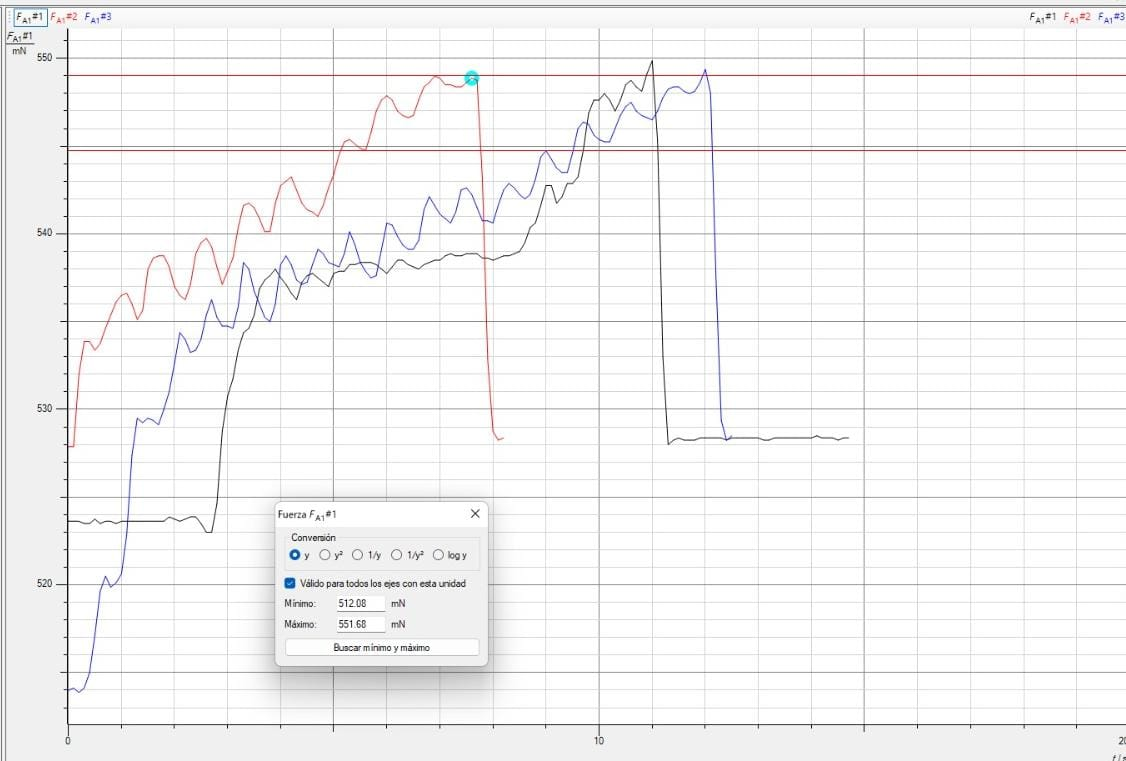
\includegraphics[width=0.8\textwidth]{../figuras/aguapura.jpeg}
    \caption{Registro de la fuerza en función del tiempo para el agua pura.}
    \label{fig:grafica_agua_pura}
\end{figure}

Utilizando la misma ecuación \eqref{eq:tension_superficial}, se procede a calcular el coeficiente de tensión superficial para el agua pura:

\begin{table}[H]
    \centering
    \label{tab:resultados_gamma_agua}
    \begin{tabular}{@{}lcc@{}}
        \toprule
        \textbf{Curva} & \textbf{\(\Delta F\) (N)} & \textbf{\(\gamma\) (N/m)} \\ \midrule
        Negra & 0.026250 & 0.0351 \\
        Roja  & 0.021125 & 0.0283 \\
        Azul  & 0.035375 & 0.0473 \\ \midrule
        \textbf{Promedio} & - & \textbf{0.0369} \\ \bottomrule
    \end{tabular}
        \caption{Cálculo del coeficiente de tensión superficial para el agua pura.}

\end{table}

El valor promedio experimental obtenido para la tensión superficial del agua pura es de \(\gamma \approx 0.0369 \text{ N/m}\) (o \(36.9 \text{ mN/m}\)). 





\subsection{Cálculo de incertidumbres por propagación de errores}

Para determinar la confiabilidad de los valores obtenidos, se aplicó el método de propagación de errores. Las variables que intervienen en el cálculo de la tensión superficial son la fuerza neta (\(\Delta F = F_{max} - F_{inicial}\)) y el perímetro de contacto (\(L\)). Sus incertidumbres absolutas se definen a continuación:

\begin{itemize}
    \item \textbf{Incertidumbre del perímetro (\(\Delta L\)):} Las mediciones de los diámetros con el calibrador (precisión de \(0.05 \text{ mm}\)) se propagan como una suma: 
    \(\Delta L = \pi (\Delta d_{ext} + \Delta d_{int}) = \pi(0.05 + 0.05) \text{ mm} = 0.314 \text{ mm} = 0.000314 \text{ m}\).
    \item \textbf{Incertidumbre de la fuerza (\(\Delta (\Delta F)\)):} El sensor de fuerza Leybold tiene una precisión de \(\pm 0.1 \text{ mN}\). Como \(\Delta F\) es una diferencia de dos lecturas (máxima e inicial), la incertidumbre combinada es \(\Delta (\Delta F) = \sqrt{2} \cdot 0.1 \text{ mN} \approx 0.1414 \text{ mN} = 1.414 \times 10^{-4} \text{ N}\).
\end{itemize}

A continuación se determinará la incertidumbre para cada caso usando la ecuación \eqref{eq:propagacion}:


\subsubsection{Incertidumbre del agua pura}

A modo de ejemplo, para la medición de la curva negra (\(\Delta F = 0.02625 \text{ N}\), \(\gamma = 0.0351 \text{ N/m}\), \(L = 0.37385 \text{ m}\)):
\begin{align*}
    \frac{\Delta (\Delta F)}{\Delta F} &= \frac{1.414 \times 10^{-4}}{0.02625} \approx 0.00539 \\
    \frac{\Delta L}{L} &= \frac{0.000314}{0.37385} \approx 0.00084 \\
    \Delta \gamma &= 0.0351 \cdot \sqrt{(0.00539)^2 + (0.00084)^2} \\
    \Delta \gamma &= 0.0351 \cdot \sqrt{2.905 \times 10^{-5} + 7.056 \times 10^{-7}} \\
    \Delta \gamma &\approx 0.0351 \cdot 0.00545 \approx \mathbf{0.00019 \text{ N/m}}
\end{align*}

Por lo tanto, el valor de la tensión superficial para esta curva se reporta como:
\begin{equation*}
    \gamma = (0.0351 \pm 0.0002) \text{ N/m}
\end{equation*}

Aplicando el mismo procedimiento para las tres curvas de agua pura, se obtienen los siguientes resultados con sus respectivas incertidumbres:

\begin{table}[H]
    \centering
    \label{tab:resultados_incertidumbre}
    \begin{tabular}{@{}lccc@{}}
        \toprule
        \textbf{Curva} & \textbf{\(\gamma\) (N/m)} & \textbf{\(\Delta \gamma\) (N/m)} & \textbf{Resultado final} \\ \midrule
        Negra & 0.0351 & 0.0002 & \((0.0351 \pm 0.0002) \text{ N/m}\) \\
        Roja  & 0.0283 & 0.0002 & \((0.0283 \pm 0.0002) \text{ N/m}\) \\
        Azul  & 0.0473 & 0.0003 & \((0.0473 \pm 0.0003) \text{ N/m}\) \\ \bottomrule
    \end{tabular}
    \caption{Resultados finales con incertidumbre por propagación de errores para el agua pura.}

\end{table}

Dado que los valores de las tres curvas presentan una dispersión mayor que la incertidumbre instrumental individual, se calculó la incertidumbre del valor promedio del agua pura:

\begin{equation*}
    \Delta \gamma_{prom} = \frac{S}{\sqrt{n}} = \frac{0.0096}{\sqrt{3}} \approx 0.0055 \text{ N/m}
\end{equation*}

Por lo tanto, el resultado experimental final para la tensión superficial del agua pura, considerando la dispersión de las mediciones, es:
\begin{equation}
    \gamma_{agua} = \mathbf{(0.037 \pm 0.006) \text{ N/m}}
\end{equation}

\subsection{Incertidumbre para el agua con detergente}

Siguiendo el mismo procedimiento de propagación de errores descrito en la sección anterior, se calcularon las incertidumbres para las mediciones del agua con detergente. 

A modo de ejemplo, para la medición de la \textbf{curva negra de agua con detergente} (\(\Delta F = 0.010625 \text{ N}\), \(\gamma = 0.0142 \text{ N/m}\)):

\begin{align*}
    \frac{\Delta (\Delta F)}{\Delta F} &= \frac{1.414 \times 10^{-4}}{0.010625} \approx 0.01331 \\
    \frac{\Delta L}{L} &= \frac{0.000314}{0.37385} \approx 0.00084 \\
    \Delta \gamma &= 0.0142 \cdot \sqrt{(0.01331)^2 + (0.00084)^2} \\
    \Delta \gamma &= 0.0142 \cdot \sqrt{1.771 \times 10^{-4} + 7.056 \times 10^{-7}} \\
    \Delta \gamma &\approx 0.0142 \cdot 0.01334 \approx \mathbf{0.00019 \text{ N/m}}
\end{align*}

Por lo tanto, el valor de la tensión superficial para esta curva se reporta como:
\begin{equation*}
    \gamma = (0.0142 \pm 0.0002) \text{ N/m}
\end{equation*}

Aplicando el mismo procedimiento para las tres curvas, se obtienen los siguientes resultados con sus respectivas incertidumbres instrumentales:

\begin{table}[H]
    \centering
    \label{tab:resultados_incertidumbre_detergente}
    \begin{tabular}{@{}lccc@{}}
        \toprule
        \textbf{Curva} & \textbf{\(\gamma\) (N/m)} & \textbf{\(\Delta \gamma\) (N/m)} & \textbf{Resultado final} \\ \midrule
        Negra & 0.0142 & 0.0002 & \((0.0142 \pm 0.0002) \text{ N/m}\) \\
        Roja  & 0.0087 & 0.0002 & \((0.0087 \pm 0.0002) \text{ N/m}\) \\
        Azul  & 0.0057 & 0.0002 & \((0.0057 \pm 0.0002) \text{ N/m}\) \\ \bottomrule
    \end{tabular}
    \caption{Resultados finales con incertidumbre por propagación de errores para el agua con detergente.}
\end{table}

Al igual que en el caso del agua pura, la dispersión de los valores experimentales es significativamente mayor que la incertidumbre instrumental. Por ello, se calculó la incertidumbre del valor promedio.
\begin{align*}
    \bar{\gamma}_{det} &= \frac{0.0142 + 0.0087 + 0.0057}{3} = 0.00953 \text{ N/m} \\
    S &= \sqrt{\frac{(0.0142-0.00953)^2 + (0.0087-0.00953)^2 + (0.0057-0.00953)^2}{2}} \approx 0.00426 \text{ N/m} \\
    \Delta \gamma_{prom} &= \frac{S}{\sqrt{n}} = \frac{0.00426}{\sqrt{3}} \approx \mathbf{0.0025 \text{ N/m}}
\end{align*}

Por lo tanto, el resultado experimental final para la tensión superficial del agua con detergente es:
\begin{equation}
    \gamma_{detergente} = \mathbf{(0.0095 \pm 0.0025) \text{ N/m}}
\end{equation}


\newpage
\section{Análisis de resultados}

A partir de los datos obtenidos experimentalmente y procesados en las secciones anteriores, se pueden extraer las siguientes observaciones físicas sobre el comportamiento de la tensión superficial:

\subsection{Efecto del agente tensioactivo (Detergente)}
La diferencia más notable entre ambas muestras analizadas es el valor del coeficiente de tensión superficial. El agua pura registró un valor promedio de \(\gamma_{agua} = (0.037 \pm 0.006) \text{ N/m}\), mientras que el agua con detergente presentó un valor de \(\gamma_{det} = (0.0095 \pm 0.0025) \text{ N/m}\). 

Esta reducción de casi cuatro veces en el valor de la tensión superficial se debe a que el detergente actúa como un agente tensioactivo. Sus moléculas se acumulan en la interfaz líquido-aire, debilitando las fuerzas de cohesión intermoleculares (puentes de hidrógeno) del agua. Como resultado, la película líquida ofrece menos resistencia a ser estirada, lo que se traduce en una menor fuerza necesaria para desprender el anillo, tal como se evidenció en los picos máximos de las gráficas de fuerza.

\subsection{Discrepancia con el valor teórico del agua pura}
El valor teórico del coeficiente de tensión superficial del agua pura a temperatura ambiente (\(20^\circ\text{C}\)) es de aproximadamente \(72 \text{ mN/m}\). Nuestro valor experimental de \(37 \text{ mN/m}\) presenta un error relativo cercano al \(48\%\). 

Si bien la incertidumbre estadística de nuestras mediciones es baja, esta gran discrepancia indica la presencia de errores sistemáticos en el montaje, como
el control cnstante de la temperatura, o una subida mas del anillo mas preciso, etc.
\subsection*{4. Comparación de los tres registros (Curvas negra, roja y azul)}
Se observó una alta dispersión entre las tres mediciones de una misma muestra. Por ejemplo, en el agua pura, la curva azul arrojó un valor de \(\gamma\) significativamente mayor (\(0.0473 \text{ N/m}\)) que la curva roja (\(0.0283 \text{ N/m}\)). Esta variabilidad demuestra la 
importancia de ser precisos al tomar datos, puesto que se hicieron varias tomas de dtaos pero solo se seleccionaron las que arrojaran datos mas contundentes.

\newpage
\section{Conclusiones}

\begin{enumerate}
    \item Se determinó experimentalmente el coeficiente de tensión superficial mediante el método del anillo de Du Noüy, obteniendo un valor para el agua pura de \(\gamma_{agua} = (0.037 \pm 0.006) \text{ N/m}\) y para la solución de agua con detergente de \(\gamma_{det} = (0.0095 \pm 0.0025) \text{ N/m}\).

    \item Se comprobó cuantitativamente el efecto de los agentes tensioactivos. La solución con detergente presentó una tensión superficial aproximadamente cuatro veces menor que el agua pura. Esto se evidenció en las gráficas de fuerza, donde el agua con detergente formó una película líquida más elástica y resistente a la ruptura antes de desprenderse del anillo.

    \item El valor experimental del agua pura (\(37 \text{ mN/m}\)) se encontró por debajo del valor teórico reportado en la literatura (\(\approx 72 \text{ mN/m}\)). Esta discrepancia se atribuye principalmente a errores sistemáticos, como la posible contaminación del anillo con residuos de detergente o grasa, y a la velocidad de elevación no cuasi-estática que introdujo fuerzas dinámicas en la medición.

    \item A pesar de la dispersión en los datos y las diferencias con los valores teóricos, el uso de la propagación de errores y la selección de las curvas más contundentes permitieron obtener resultados con un margen de incertidumbre aceptable, validando el método experimental para fines comparativos y didácticos.
\end{enumerate}

\newpage
\addcontentsline{toc}{section}{Referencias}

\begin{thebibliography}{5}
    \bibitem{serway} Serway, R. A. y Jewett, J. W. \textit{Física para ciencias e ingeniería}. Volumen 1. Cengage Learning.
    \bibitem{young} Young, H. D. y Freedman, R. A. \textit{Física universitaria}. Volumen 1. Pearson Educación.
    \bibitem{halliday} Halliday, D., Resnick, R. y Walker, J. \textit{Fundamentos de física}. Wiley.
    \bibitem{giacoli} Giancoli, D. C. \textit{Física: principios con aplicaciones}. Pearson Educación.
    \bibitem{guia} Universidad Nacional de Ingeniería. \textit{Guía de laboratorio de Física II: Tensión Superficial}. Facultad de Ciencias.
\end{thebibliography}

\newpage
\section{Anexos}

\subsection{Repositorio del proyecto}

Los códigos utilizados para el procesamiento de datos experimentales, la elaboración de las gráficas y los archivos fuente del informe se encuentran disponibles en el siguiente repositorio:

\url{https://github.com/alexandrade0z-wq/FISICA-2-LABORATORY/tree/main/Lab04}

\subsection{Participación de los integrantes}

La distribución de responsabilidades del equipo se presenta en la Tabla \ref{tab:participacion}.

\begin{table}[H]
    \centering
    \label{tab:participacion}
    \begin{tabular}{|l|l|p{7cm}|}
        \hline
        \textbf{Apellidos y nombres} & \textbf{Código} & \textbf{Responsabilidades} \\ \hline
        Moreno Cabanillas, Alexandra Romina & 20251764f & Montaje experimental, toma de datos y redacción de fundamentos teóricos. \\ \hline
        Polak Mory, Mauricio Andre & 20250575E & Procesamiento de datos, cálculo de incertidumbres y análisis de resultados. \\ \hline
        Cárdenas Loyola, Pablo Mauro & 20262378E & Elaboración de gráficas, verificación de datos y redacción de conclusiones. \\ \hline
    \end{tabular}
    \caption{Distribución de responsabilidades del equipo.}

\end{table}

Los tres integrantes participaron en la ejecución de la experiencia, la discusión de los resultados y la revisión general del informe.


\end{document}